\documentclass{IEEEtran}

\usepackage{amsmath}
\usepackage{listings}
\lstset{
    basicstyle=\small\ttfamily,
    breaklines=true
}
\usepackage{graphicx}
\graphicspath{ {./images/} }
\usepackage{xcolor}
\pagecolor[rgb]{0.1,0.1,0.1}
\color[rgb]{1,1,1}

\title{Readings about Strings and Tries}
\author{Diego Linares - kiwiAipom}

\begin{document}
  \maketitle
  \section{Manacher's Algorithm}
    \textbf{Statement:} Find all pairs $(i,j)$ which make a palyndrome substring.
    \subsection{Detailed Statement}
      Worst case we would have $O(n^2)$ palyndromes.\par 
      \textbf{Compact way of keeping palyndromes:} $i = 0\ldots n-1$, $d_1[i],d_2[i]$ represent the number of palyndromes with odd and even length with their center in $i$.\par 
      \textbf{Ex.} $abababc$, has $d_1=3$ (odd length), and $cbaabd$ has $d_2[3] = 2$ (even length). \par 
      Sub-palindrome with $l$ size with center in $i$, we also have with $l-2, l-4,\ldots$. \par 
      Both palyndrom arrays can be calculated in linear time. \par 
      \textbf{Solution:} Can be done with string hashing and suffix trees, but this has a smaller constant and memory complexity.
    \subsection{Trivial Algorithm}
      Tries to increase the answer by one until it's possible for each center $i$. It is $O(n^2)$ in time. Implementation being:
      \begin{lstlisting}
vector<int> d1(n),  d2(n);
for (int i = 0; i < n; i++) {
    d1[i] = 1; // Pair with itself 
    while (0 <= i - d1[i] && i + d1[i] < n && s[i - d1[i]] == s[i + d1[i]]) {
        d1[i]++;
    }

    d2[i] = 0;
    while (0 <= i - d2[i] - 1 && i + d2[i] < n && s[i - d2[i] - 1] == s[i + d2[i]]) {
        d2[i]++;
    }
}
      \end{lstlisting}
    \subsection{Manacher's Algorithm}
      Allows to find all the sub-palyndromes with odd length (even length is just a small mod).\par 
      \textbf{Borders:} $(l,r)$ of the palyndrome with maximal $r$. Initially we assume $l=0,r=-1$\par 
      We want to calculate $d_1[i]$ with all the previous $i$ already calculated.
      \begin{itemize}
        \item If it is ourside of the current rightmost sub-palyndrome $i > r$, we launch the trivial algorithm, allowing us to calculate $d_i[i]$ and updating $(l,r)$.
        \item $i \leq r$. We can flip $i$ into $j=l+(r-i)$ and since they are symmetrical, we can \textbf{almost always} do $d_1[i] = d_1[j]$. Like so: 
        \begin{center}
          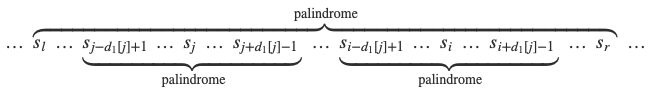
\includegraphics[width = 0.45\textwidth]{manacherIllust.png}
        \end{center}
        \item \textbf{Trick case:} When the inner palyndrome reaches the border of the outer one. $j-d_1[j]+1\leq l$. Since the symmetry of the outer palyndrome is not guaranteed, we assign $d_1[i] = r - i + 1$, and then run the trivial algorithm to increase the value if necessary, updating in the end. Like so:
        \begin{center}
          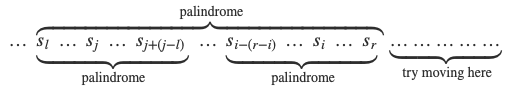
\includegraphics[width=0.45\textwidth]{manacherTrick.png}
        \end{center}
        \par Note we only use the part of the palyndrome with guaranteed symmetry before moving to the \textit{try moving here part}. 
      \end{itemize}
      \par A similar algorithm is then used for the even part.
    \subsection{Complexity}
      Not as intuitive, but if we look at \textit{Z-function building algorithm} we can check it's similar and linear. \par 
      We can also notice that $r$ can only increase by one ine very iteration of the trivial algorithm, and that it can't decrease. $O(n)$ iterations. The rest is linear.
    \subsection{Implementation}
      Here is the implementation, which is fairly similar for both $d_1,d_2$.
      \begin{lstlisting}
vector<int> d1(n), d_2(n);
for (int i = 0, l = 0, r = -1; i < n; i++) {
    int k = (i > r) ? 1 : min(d1[l + r - i], r - i + 1);
    while (0 <= i - k && i + k < n && s[i - k] == s[i + k]) {
        k++;
    }
    d1[i] = k--;
    if (i + k > r) {
        l = i - k;
        r = i + k;
    }
}
for (int i = 0, l = 0, r = -1; i < n; i++) {
    int k = (i > r) ? 0 : min(d2[l + r - i + 1], r - i + 1);
    while (0 <= i - k - 1 && i + k < n && s[i - k - 1] == s[i + k]) {
        k++;
    }
    d2[i] = k--;
    if (i + k > r) {
        l = i - k - 1;
        r = i + k ;
    }
}
      \end{lstlisting}
  \section{Z-function}
    String $s$ of length $n$. The function returns an array of length $n$ where $Z[i]$ is equal to \textbf{greatest number of characters starting from position $i$, that coincide with the first characters of $s$}. Longest common prefix between $s$, and suffix of $s$ starting at $i$.\par 
    We assume 0 based indexing and $z[0]=0$. It is $O(n)$ time. \par 
    \textbf{Ex.} $aaaaa=[0,4,3,2,1], aaabaab=[0,2,1,0,2,1,0], abacaba=[0,0,1,0,3,0,1]$. \par 
    \subsection{Trivial Algorithm}
      This one is $O(n^2)$: 
      \begin{lstlisting}
vector<int> z_function_trivial(string s) {
    int n = (int) s.length();
    vector<int> z(n);
    for (int i = 1; i < n; ++i)
        while (i + z[i] < n && s[z[i]] == s[i + z[i]])
            ++z[i];
    return z;
}
      \end{lstlisting}
      Basically calculating $z[i]$ for each $i$ independently.
    \subsection{Efficient} 
      We make use of the previously computed values. \par 
      \textbf{Segment Match:} a substring which coincides with a prefix of $s$. So $z[i]$ is the length of the segment match that starts at $i$ at ends at $i+z[i]-1$.\par 
      $(l,r)$ will be the indices of our rightmost segment match. $r$ can be seen as the boundary to which our string has been scanned by the algorithm.\par 
      If we are in index $i$, there are two options to calculate: 
      \begin{itemize}
        \item $i>r$, so we haven't processed the current position yet. So we run the trivial algorithm. If $z[i]>0$ we have to update $r = i + z[i] - 1$.
        \item Otherwise, we are inside the current segment match. We can use the previou values to give us a head start, through the value $z[i-l]$, since $s{l..r}$ and $s[0..l-r]$ match.\par 
        However, the value might be too large, and when applied to $i$ we could get an overflow. For example $aaaabaa$, in $i=6$ we are not able to initialize it with $z[1]=3$ since we would overflow the array. So we instead do:
        $$z_0[i]=min(r-i+1,z[i-l])$$
        \par Then we increment $z[i]$ with the trivial algorithm, to see if it continues to match or not.
      \end{itemize}
      The only difference between the cases is the initial value of $z[i]$, then both branches use the trivial algorithm. 
    \subsection{Implementation}
      \begin{lstlisting}
vector<int> z_function(string s) {
  int n = (int) s.length();
  vector<int> z(n);
  for (int i = 1, l = 0, r = 0; i < n; ++i) {
    if (i <= r)
      z[i] = min (r - i + 1, z[i - l]);
    while (i + z[i] < n && s[z[i]] == s[i + z[i]])
      ++z[i];
    if (i + z[i] - 1 > r)
      l = i, r = i + z[i] - 1;
  }
  return z;
}
      \end{lstlisting}
      \par Returns an array of size $n$. \par
      The initial array is initially filled with $0$ and the rightmost match is $[0,0]$. We then first check what option of the algorithm we are gonna use, and in the end if necessary, we update the rightmost segment ($i + z[i] - 1 > r$).
    \subsection{Asymptotic Behavior}
      It's $O(n)$, and we only need to focus on the \texttt{while} loop, showing that each iteration will increase the right border $r$. So we consider both branches of the algorithm.
      \begin{itemize}
        \item $i>r$: If $s[0] \neq s[i]$ it won't make any iterations, otherwise it will necessarily move to the right and update $r$.
        \item $i\leq r$. We initialize $z[i]$ to $z_0$, and we need to compare this to $r - i + 1$ so we have a trichotomy:
        \begin{itemize}
          \item $z_0 < r-i+1$: No iteration of the loop will take place. If it did, the initial $z_0$ approximation was inaccurate. But that is not true because we know $s[l..r]$ and $s[0...r-l]$ match.
          \item $z_0 = r-i+1$: In this case, it will make a few iterations, but each will lead to an increase of $r$ since we will start comparing from $s[r+1]$ increasing the $(l,r)$ interval.
          \item $z_0 > r-i+1$: By definition, can't happen.
        \end{itemize}
      \end{itemize}
      Each iteration of the inner loop makes $r$ increase, and at most $n-1$ times, since it won't be able to overflow the array. \par 
      The rest of the algorithm clearly runs in $O(n)$ so it is proven. 
    \subsection{Applications}
      Very similar to the prefix function ones.
      \subsubsection{Search the Substring}
        Find all the ocurrences of a pattern $p$ inside a text $t$. \par 
        We create a new string $p+\alpha+t$, $\alpha$ being a separator character we are sure won't appear. \par 
        Compute the function for this string, then for every $i$ in the range $[0;length(t)-1]$ consider the corresponding value.
        $$k = z[i+length(p)+1]$$
        \par If $k$ is equal to $length(p)$ we know there is one ocurrence in the $i$ position of the text. \par 
        Running time and memory consumption of $O(length(t)+length(p))$
      \subsubsection{Number of distinct substrings}
        \textbf{Iterative approach:} Knowing the current number of different substrigns, recalculate after adding the end of $s$ one character.\par 
        $k$ being the current number, we add $c$ to $s$. There can be new substrings which end in $c$ (all the ones that end with this symbol and we haven't encountered yet).\par 
        Take a string $t=s+c$ and invert it. So, now we have to count how many prefixes in $t$ are not found anywhere else in $t$.\par 
        Compute the Z-function of $t$ and find its max value, $z_{max}$. The number of new substrings that appear when symbol $c$ is appended to $s$ is equal to:
        $$length(t)-z_{max}$$
        \par Running time being $O(n^2)$
        We can recalculate in $O(n)$ time the amount of substrings when adding at the beginning and removing.
      \subsubsection{String Compression}
        In $s$ find a string $t$ of shortest length, such that $s$ can be represented as concatenations of $t$.\par 
        \textbf{Z-function solution:} compute de function of $s$ loop through all $i$ which divide $n$, stop at the first $i$ such that $i+z[i]=n$. The string then can be compressed to length $i$.\par 
        Can also be done with prefix function, check that for the proof. 
  \begin{thebibliography}{}
    \bibitem{manacher}
      \textit{Manacher's Algorithm - Finding all sub-palindromes in $O(N)$},
      jakobkogler for E-maxx.
      From: https://cp-algorithms.com/string/manacher.html
    \bibitem{zfunction}
      \textit{Z-function and its calculation},
      E-maxx.
      From: https://cp-algorithms.com/string/z-function.html
  \end{thebibliography}
\end{document}
